\chapter{Implementation}

\section{Problem Statement}

This case study aims on to make the inversion of a single-element feedforward neural network. However the implementation of the inversion is just the last step during the process, due to it needs a lot of preprocessing to make the appropriate model.\medskip

This work belongs in the realm of machine learning application research. There are three main tasks examinated in this paper: data mining for extracting information from a data set, building and testing multilayer perceptron models for, and inverting these feedforward neural network models. \bigskip

The first task is to choose a dataset which contains usable data. The selected one is called the Online News Popularity Dataset by Mashable news, that was served by the  \href{http://archive.ics.uci.edu/ml/datasets/Online+News+Popularity}{UCI's Machine Learning Repository}. \smallskip

The dataset is preprocessed by Pandas to a DataDrame to be ready for data mining. Since being a publicly available dataset, its preprocessing and transformation has already made, but the dataset even needs some cleaning with the assistance of Scikit-Learn. The dataset contains a lot of outlying values that should be handled, and the dataset necessiates a standard scaling. Furthermore as the dataset is large-scaled, the less important features are simply removed. Then the dataset can be splitted into training and testing sets by Scikit-Learn. \medskip

The training phase consists of the application of machine learning techniques. Different multi-layer perceptron models are fitted on the training set with various parameters. These attributes changed in their hidden layer sizes, activation functions, optimization algorithms, learning rate sizes and alpha values. With the utilization of the inputs, Scikit-Learn trains the training dataset and make predictions to the testing set. The training is very time consuming, since the used dataset is very large, and also the length is depending on the amount of attributes of multi-layer perceptron models. In the end of each process, the testing set's output and the predicted output are compared and the difference between them is calculated. If all of the iterations are ended, the best estimator's parameters are shown with its score, and the tested target values and the predicted ones are plotted by Matplotlib.\medskip

From the results of the training, the single-element inversion can be performed by Scikit-Learn. It is an iterative process, where the target values are the new predictors with the knowledge comes from the other features. Every iteration calculates one single feature's values and the accuracy between the feature's original and the calculated values. The results are also plotted by Matplotlib. \medskip

These results show the influence of the features to the target. The larger the score, the more important the feature is.



\subsection{Used Third-Party Libraries}

Python can be used effectively with the assistance of some of its third-party libraries \cite{g2015learning} \cite{bressert2012scipy}, which provide numerous effective and easy-to-use models in scientific research. \bigskip

\textbf{Pandas} \cite{chen2017pandas} is an open source library providing high-performance, easy-to-use data structures and data analysis tools for Python. Pandas has a main object called DataFrame, that is for data manipulation using a set of labeled array data structures. Pandas has tools for reading tabular data and writing data between in-memory data structures and different file formats. The data can be handled integratedly and the data sets are transformable. Some of the examples of this transformation are column insertion and deleting, data set merging and joining, or the hierarchical axis indexing in high-dimensional data models.\bigskip


\textbf{Matplotlib} is an open source Python library that produces publication-quality plots and figures. It ships with several add-on toolkits, including 3d plotting and assistance for axes. There are several common approaches of plotting in Matplotlib. The most popular is $pyplot$, which is a collection of command style functions where each $pyplot$ function makes some change to a figure. Also it is mainly intended for interactive plots and simple cases of programmatic plot generation.


\subsubsection{Scikit-Learn}

The most important package that is used during the implementation is Scikit-Learn. It is a separately-developed and distributed third-party extension to SciPy. It integrates classic machine learning algorithms into the scientific Python packages. \smallskip

Scikit-Learn can be used to solve multi-layer neural network learning problems. Among many others, it features various classification, regression and clustering algorithms. Scikit-Learn contains all the various functions which can be used during the training of the neural network. The training lasts from the processing of the data set, via the iterations, to the inversion itself. \bigskip

\textbf{StandardScaler} is a subclass of Scikit-Learn's prepropressing class that standardizes features by removing the mean and scaling to unit variance. It has three parameters that are boolen values and the default of all is True: \smallskip

\noindent - $copy$ means if the original dataset will be replaced with the scaled one or not\\
- $with\char`_mean$ means if the scaler centers the data before scaling or not\\
- $with\char`_std$ means if the data is scaled to unit variance or not \medskip

The standard score of a sample $x$ is calculated as: $z = \frac{(x - u)}{s}$ where $u$ is the mean of the training samples or zero if $with\char`_mean=False$, and $s$ is the standard deviation of the training samples or one if $with\char`_std=False$. \medskip

\noindent StandardScaler has some methods:
\begin{verse}
	$\bullet$ $fit(X[, y])$ computes the mean and the standard deviation to be used for later scaling\\
	$\bullet$ $fit\char`_transform(X[, y])$ fits to data, then transforms it\\
	$\bullet$ $get\char`_params([deep])$ gets parameters for this estimator\\
	$\bullet$ $inverse\char`_transform(X[, copy])$ scales back the data to the original representation\\
	$\bullet$ $partial\char`_fit(X[, y])$ is the online computation of mean and standard deviation on $X$ for later scaling\\
	$\bullet$ $set\char`_params(**params)$ sets the parameters of this estimator\\
	$\bullet$ $transform(X[, y, copy])$ performs standardization by centering and scaling
\end{verse}\smallskip

\textbf{Train\char`_test\char`_split} is a subclass of Scikit Learn's selection class, which splits arrays or matrices into random train and test subsets. The randomization is important in ordered data sets. Allowed inputs are lists, NumPy arrays, SciPy-sparse matrices or Pandas DataFrames. Train\char`_test\char`_split returns with four lists that contains the train-test splits of inputs.\medskip

\noindent The parameters are the following:\smallskip

\noindent - $test\char`_size$ : If $float$, it should be between 0.0 and 1.0 and represents the proportion of the dataset to include in the test split. If $int$, it represents the absolute number of test samples. If $None$, the value is set to the complement of the train size. \\
- $train\char`_size$ : If $float$, it should be between 0.0 and 1.0 and represents the proportion of the dataset to include in the train split. If $int$, it represents the absolute number of train samples. If $None$, the value is automatically set to the complement of the test size.\\
- $random\char`_state$ : If $int$, it is the seed used by the random number generator. If $RandomState$ instance, it is the random number generator. If $None$, the random number generator is the $RandomState$ instance used by $np.random$.\\
- $shuffle$ : Whether or not to shuffle the data before splitting.\\
- $stratify$ : It shows if the data is split in a stratified fashion, using this as the class labels.\bigskip


\textbf{MLPRegressor} \cite{bengfort2018applied} is a class of Scikit-Learn, which implements a multi-layer perceptron, that uses the square error as the loss function. It trains iteratively because the partial derivatives of the loss function are computed in each step to update the parameters of the layers. MLPRegressor also supports multi-output regression, in which a sample can have more than one target outputs.\medskip

\noindent MLPRegressor has several parameters, but only a few of them will be listed, which were used in the implementation:
\begin{verse}
	$\bullet$ $hidden\char`_layer\char`_sizes$ is a tuple where the $i$th element represents the number of neurons in the ith hidden layer.
	
	$\bullet$ $activation$ is the activation function for the hidden layer.\\
	\hspace{10pt} - ‘identity’ provides the linear function, returns $f(x) = x$\\
	\hspace{10pt} - ‘logistic’ provides the logistic sigmoid function, returns $f(x) = \frac{1}{1 + e^{-x}}.$\\
	\hspace{10pt} - ‘relu’ provides the rectified linear unit function, returns $f(x) = max(0, x)$. \\
	\hspace{10pt} - ‘tanh’ provides the hyperbolic tan function, returns $f(x) = tanh(x)$.
	
	$\bullet solver$ is the optimization algorithm used in weight optimization.\\
	\hspace{10pt} - ‘sgd’ refers to stochastic gradient descent.\\
	\hspace{10pt} - ‘adam’ refers to a transition between adaptive methods and momentum-based methods.\\
	\hspace{10pt} - ‘lbfgs’ is an optimizer in the family of quasi-Newton methods.
	
	$\bullet alpha$ is the L2 regularization parameter's value.
	
	$\bullet learning\char`_rate\char`_init$ is the initial learning rate that is used. It controls the step-size in updating the weights. Only used when the solver is $sgd$ or $adam$.
	
	$\bullet learning\char`_rate$ means the learning rate schedule for weight updates. \\
	\hspace{10pt} - ‘constant’ is a constant learning rate given by $learning\char`_rate\char`_init$.\\
	\hspace{10pt} - ‘invscaling’ gradually decreases the learning rate at each time step using an inverse scaling exponent.\\
	\hspace{10pt} - ‘adaptive’ keeps the learning rate constant as long as training loss keeps decreasing.
\end{verse}
MLPRegressor contains built-in methods to perform regression:\\
- $fit(X, y)$ fits the model to data matrix $X$ and target(s) $y$.\\
- $get\char`_params([deep])$ gets parameters for this estimator.\\
- $predict(X)$ predicts an output based on previous training and a given testing dataset.\\
- $score(X, y[, sample\char`_weight])$ returns with the coefficient of the determinated prediction.\\
- $set\char`_params(^{**} params)$ sets the parameters of the estimator.\bigskip


\textbf{GridSearchCV} is an exhaustive searching class of Scikit-Learn over specified parameter values for an estimator. It can be used in the tuning of the hyper-parameters, which are those parameters that are not directly learnt within estimators. The parameters of the estimator used to apply the methods of GridSearchCV are optimized by cross-validated grid-search over a parameter grid.\medskip

\noindent The parameters of GridSearchCV are quite wide, but only a few of them are used during the implementation:
\begin{verse}
	$\bullet estimator$ implements the estimator interface. \\
	$\bullet param\char`_grid$ is a dictionary with the names of the used parameters as keys and lists of parameter settings to try as values\\
	$\bullet cv$ is an integer that determines the cross-validation splitting strategy
\end{verse}

From GridSearchCV's attributes, $best\char`_params\char`_$ is used, which is a dictionary about the parameter setting that gave the best results on the hold out data.\medskip

\noindent GridSearchCV contains built-in methods for prediction:\\
- $fit(X[, y, groups])$ method fits with the adjusted parameter grid on the given dataset.\\
- $get\char`_params([deep])$ gets parameters for this estimator.\\
- $predict(X)$, $predict\char`_log\char`_proba(X)$ and $predict\char`_proba(X)$ make the prediction on the test set\\
- $score(X[, y])$ returns the score on the given data, if the estimator has been refit.\\
- $set\char`_params(**params)$ sets the parameters of this estimator.\bigskip


\section{The Implementation}

The first step was to import all of the necessary libraries.
\begin{lstlisting}
import pandas as pd
import matplotlib.pyplot as plt
from sklearn.preprocessing import StandardScaler
from sklearn.model_selection import train_test_split
from sklearn.model_selection import GridSearchCV
from sklearn.neural_network import MLPRegressor
\end{lstlisting}

After, the selected dataset has captured by Pandas. In this case the used dataset is a .csv file, which contains 39644 instances and 61 attributes. The attributes consist of 58 predictive features, 2 other attributes of accessory information and 1 goal field, which is the number of shares. The dataset represents as a matrix, where the columns are the features and the rows are the datas. This dataset is preprocessed by Pandas as a DataFrame object. The $url$ and $timedelta$ columns have been omitted, since they are meta-data and cannot be treated as features. 
\begin{lstlisting}
dataset = pd.read_csv('OnlineNewsPopularity.csv')
dataset_copy = dataset.drop(columns=['url','timedelta'])
\end{lstlisting}

\medskip As already mentioned, the dataset's preprocessing and transformation has made, but the dataset even needs some cleaning. Before doing that, let's give a check on the summarization:
\begin{lstlisting}
dataset_copy.describe()
\end{lstlisting}
where the first 5 columns results the following:
\begin{figure}[h]
	\centering
	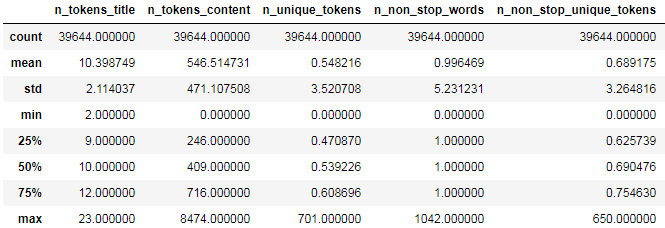
\includegraphics[height=0.34\linewidth]{./figures/describe1}
	\caption{A part of the summarization of the initial dataset}
	\label{fig:describe1}
\end{figure}

\noindent As it can be seen in the table, there are outlier values that would cause noise if they will not be handled. Also, in the known of the meaning of each columns, some inconsistencies are occured, like the $n\char`_tokens\char`_content$ feature contains the number of words in the content, which cannot be zero. These inconsistent values needs a correction.


\subsection{Optimizing the Dataset}

There are a lot of techniques in data mining for optimizing the datas into appropriate forms. In the case of outlying and inconsistent values, due to the huge number of datas, the chosen technique was to simply ignore those tuples. 
\begin{lstlisting}
dataset_copy = dataset_copy[dataset_copy.n_tokens_content != 0]
dataset_copy = dataset_copy[dataset_copy.n_unique_tokens <= 1]
dataset_copy = dataset_copy[dataset_copy.average_token_length != 0]

dataset_copy = dataset_copy[dataset_copy.num_hrefs <= 100]
dataset_copy = dataset_copy[dataset_copy.num_self_hrefs <= 10]
dataset_copy = dataset_copy[dataset_copy.num_imgs <= 10]
dataset_copy = dataset_copy[dataset_copy.num_videos <= 2]
dataset_copy = dataset_copy.reset_index(drop=True)
\end{lstlisting}

These reductions need some explanation. As mentioned above, $n\char`_tokens\char`_content$ is the number of words in the content, so it cannot be zero. $n\char`_unique\char`_tokens$ contains the rate of unique words in the content. Due to it is a rate, it need to be between [0,1]. $average\char`_token\char`_length$ contains the average length of the words in the content, which also cannot be zero. \smallskip

The other optimizations are for handling the outlying values. $num\char`_hrefs$ contains the number of links, $num\char`_self\char`_hrefs$ is the number of links to other articles published by Mashable, $num\char`_imgs$ has the number of images and $num\char`_videos$ stands for the number of videos. Furthermore because this dataset is a Pandas DataFrame and $drop$ is a function for removing the whole row, the dataset needs to be reindexed.\medskip

After the cleaning, the dataset's other part is still has a big difference between its values, so the whole dataset should be scaled. 
\begin{lstlisting}
scaler = StandardScaler()
dataset_copy[:] = scaler.fit_transform(dataset_copy[:])
\end{lstlisting}
With the usage of StandardScaler's $fit\char`_transform$ method, the dataset has been fitted and transformed in one step. \medskip

\noindent Then the dataset has separated into feature $X$ and target $y$ groups.
\begin{lstlisting}
y = dataset_copy.get(key='shares').values
X = dataset_copy.drop(columns='shares').values
\end{lstlisting}
The column $shares$ contains the target values which are the number of shares.\medskip

Learning the parameters of a prediction function and testing it on the same data is a methodological mistake: a model that would just repeat the labels of the samples that it has just seen would have a perfect score but would fail to predict anything useful on yet-unseen data. This situation is called overfitting. To avoid it, it is a common practice when performing a supervised machine learning experiment to hold out a part of the available data as a testing set $X\char`_test$, $y\char`_test$. 
\begin{lstlisting}
X_train, X_test, y_train, y_test = train_test_split(X, y, test_size=0.3, random_state=0)
\end{lstlisting}
Now the training ($X\char`_train$, $X\char`_test$) and testing ($y\char`_train$, $y\char`_test$) sets are made. The $test\char`_size$ is a float, which means the testing sets have this proportion from the dataset.



\subsection{Training the Neural Network}

Now the dataset is ready to be trained. The training consists of the application of machine learning techniques. Different multi-layer perceptron models are fitted on the training sets with a set of parameters $param\char`_grid$. These parameters are the number of hidden layers, the activation functions, the optimization algorithms, the alpha value, the learning rate's type and the learning rate's initialize value. Scikit-Learn's training toolkit is called MLPRegressor, which is used as an estimator of GridSearchCV. The process of the training fits the neural network model to the training sets, then tests the accuracy on the testing sets by predicting the output $y\char`_pred$.  
\begin{lstlisting}
mlp = MLPRegressor()
param_grid = {
	'hidden_layer_sizes': [(30, 90, 180, 90, 30)],
	'activation': ['logistic', 'tanh', 'relu'],
	'solver': ['lbfgs','sgd', 'adam'],
	'alpha': [0.03, 0.01, 0.003, 0.001, 0.0003, 0.0001],
	'learning_rate_init': [0.03, 0.01, 0.003, 0.001, 0.0003, 0.0001],
	'learning_rate': ['adaptive'],
}
gs = GridSearchCV(mlp, param_grid, cv=2)
gs.fit(X_train, y_train)
y_pred = gs.predict(X_test)
\end{lstlisting}
This process is very time consuming due to the amount of the given parameters are trained on the large-scale dataset. After the trained multi-layer perceptron is ready, the results can be stored and the
received values can be plotted by Matplotlib. The score was computed by the L2 norm of the loss function, which means the difference between the original and the predicted value.
\begin{lstlisting}
print(gs.best_params_)
print(gs.score(X_test, y_test))
print('shares', gs.best_params_, gs.score(X_test,y_test), sep='; ', file=open('InversionResults.txt', 'a'))

plt.plot(X_test, y_test, 'o', color='blue')
plt.plot(X_test, y_pred, 'o', color='orange')
plt.savefig('plots/' + 'shares_prediction.pdf')
plt.show()
\end{lstlisting}

\bigskip The results of the training are the following where the original values are colored blue and the predicted ones have color orange:
\begin{figure}[h]
	\centering
	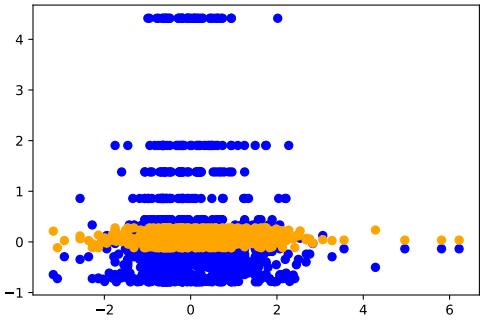
\includegraphics[height=0.378\linewidth]{./figures/shares_prediction}
	\caption{The result of the best prediction}
	\label{fig:shares}
\end{figure}

\begin{lstlisting}
shares; {'activation': 'relu', 'alpha': 0.001, 'hidden_layer_sizes': (30, 90, 180, 90, 30), 'learning_rate': 'adaptive', 'learning_rate_init': 0.0001, 'solver': 'sgd'}; 0.01229680126603272
\end{lstlisting}
which means, the score was $0.01229680126603272$ and the best estimator parameters were the ReLU activation function and SGD as optimization algorithm, with the use of $0.001$ alpha value and $0.0001$ initial learning rate. \medskip

This really bad score does not mean that the model will be bad at inversion, due to the inversion will show the importance of every single feature to the target. The reason is very simple. The WLK inversion works as the backpropagation algorithm, which means it contains a recursive equation whose iteration for inversion can be solved by computing its derivative. It can be imagined by if the WLK inversion has a forward phase that contains a fitting algorithm where the derivatives are computed and a backward phase where the recursion is computed by the derivatives. These values makes the new outputs that will be the result of the inversion.


\subsection{Inverting the MLP}


The inversion is an iterative process, which lasts for very long. Here the target values are the new predictors $X\char`_inverse$ with the knowledge comes from the other features $X$. Every iteration calculates one single feature's values $y\char`_inverse$ and also its accuracy between the feature's original and the calculated values. \medskip

The new training ($X\char`_inverse\char`_train$, $X\char`_inverse\char`_test$) and testing ($y\char`_inverse\char`_train$, $y\char`_inverse\char`_test$) sets has to be made first.
\begin{lstlisting}
X = pd.DataFrame(X)
X.columns = dataset_copy.drop(columns='shares').columns

for X_value in X:
	X_inverse = X.drop(columns=X_value).values
	X_inverse_help = pd.DataFrame(y_train)
	y_pred = pd.DataFrame(y_pred)

	for y_pred_value in y_pred.values:
		y_pred_value = pd.Series(y_pred_value)
		X_inverse_help = X_inverse_help.append(y_pred_value, ignore_index=True)
		
	X_inverse = pd.DataFrame(X_inverse)
	X_inverse.insert(0,'shares',X_inverse_help)
	X_inverse = X_inverse.values

	y_inverse = X.get(key=X_value).values


	X_inverse_train, X_inverse_test, y_inverse_train, y_inverse_test = train_test_split(X_inverse, y_inverse, test_size=0.3, random_state=0)


	[...]
\end{lstlisting}
Then the predictions can be made by fitting the multi-layer perceptron model with the same parameters as during the training phase. This is an  important step to get the appropriate inversion values.
\begin{lstlisting}
X = pd.DataFrame(X)
X.columns = dataset_copy.drop(columns='shares').columns

for X_value in X:
	X_inverse = X.drop(columns=X_value).values
	X_inverse_help = pd.DataFrame(y_train)
	y_pred = pd.DataFrame(y_pred)

	for y_pred_value in y_pred.values:
		y_pred_value = pd.Series(y_pred_value)
		X_inverse_help = X_inverse_help.append(y_pred_value, ignore_index=True)

	X_inverse = pd.DataFrame(X_inverse)
	X_inverse.insert(0,'shares',X_inverse_help)
	X_inverse = X_inverse.values

	y_inverse = X.get(key=X_value).values


	X_inverse_train, X_inverse_test, y_inverse_train, y_inverse_test = train_test_split(X_inverse, y_inverse, test_size=0.3, random_state=0)

	gs.fit(X_inverse_train, y_inverse_train)
	y_inverse_pred = gs.predict(X_inverse_test)

	print(gs.best_params_)
	print(gs.score(X_inverse_test, y_inverse_test))
	print(X_value, gs.best_params_, gs.score(X_inverse_test,y_inverse_test), sep='; ', file=open('InversionResults.txt', 'a'))

	plt.plot(X_inverse_test, y_inverse_test, 'o', color='blue')
	plt.plot(X_inverse_test, y_inverse_pred, 'o', color='orange')
	plt.savefig('plots/' + str(X_value) + '_prediction.pdf')
	plt.show()
\end{lstlisting}
In the end of each process, the resulted score and the parameters that was used for the best prediction are written to a file. Furthermore the original values of the features and the inverted ones are plotted.



\section{Results}

The obtained results helps to understand the operation of the Online News Popularity dataset. The inversion revealed the extent of how features affect the number of shares one by one. Those features that converge the most to 1, have the greatest influence.\medskip

These features's scores resulted at least 0.95 accuracy which means, these features affect the number of shares the most.
\begin{lstlisting}
kw_max_max; {'activation': 'tanh', 'alpha': 0.01, 'hidden_layer_sizes': (30, 90, 180, 90, 30), 'learning_rate': 'adaptive', 'learning_rate_init': 0.01, 'solver': 'lbfgs'}; 0.999283661233451
LDA_04; {'activation': 'tanh', 'alpha': 0.01, 'hidden_layer_sizes': (30, 90, 180, 90, 30), 'learning_rate': 'adaptive', 'learning_rate_init': 0.001, 'solver': 'lbfgs'}; 0.9978949301566046
kw_min_min; {'activation': 'tanh', 'alpha': 0.01, 'hidden_layer_sizes': (30, 90, 180, 90, 30), 'learning_rate': 'adaptive', 'learning_rate_init': 0.01, 'solver': 'lbfgs'}; 0.9978265596014307
LDA_00; {'activation': 'tanh', 'alpha': 0.01, 'hidden_layer_sizes': (30, 90, 180, 90, 30), 'learning_rate': 'adaptive', 'learning_rate_init': 0.01, 'solver': 'lbfgs'}; 0.989874004275313
rate_positive_words; {'activation': 'tanh', 'alpha': 0.01, 'hidden_layer_sizes': (30, 90, 180, 90, 30), 'learning_rate': 'adaptive', 'learning_rate_init': 0.001, 'solver': 'lbfgs'}; 0.9858555965431666
rate_negative_words; {'activation': 'tanh', 'alpha': 0.01, 'hidden_layer_sizes': (30, 90, 180, 90, 30), 'learning_rate': 'adaptive', 'learning_rate_init': 0.001, 'solver': 'lbfgs'}; 0.9827638672011125
LDA_03; {'activation': 'tanh', 'alpha': 0.01, 'hidden_layer_sizes': (30, 90, 180, 90, 30), 'learning_rate': 'adaptive', 'learning_rate_init': 0.0001, 'solver': 'lbfgs'}; 0.9631754471905054
self_reference_avg_sharess; {'activation': 'tanh', 'alpha': 0.01, 'hidden_layer_sizes': (30, 90, 180, 90, 30), 'learning_rate': 'adaptive', 'learning_rate_init': 0.0001, 'solver': 'lbfgs'}; 0.9583727915872209
\end{lstlisting}
The value of $kw\char`_max\char`_max$ is computed from ranking all article keyword maximum shares (known before publication) in order to get the best keywords. Also, $kw\char`_min\char`_min$ is the worst keyword from the ranking of minimum shared articles. $LDA\char`_04$, $LDA\char`_00$ and $LDA\char`_03$ are computed by the Latent Dirichlet Allocation algorithm, which identified the top relevant topics and then measure the closeness of current article to such topics. The $rate\char`_positive\char`_words$ is the rate of positive words among non-neutral tokens and $rate\char`_negative\char`_words$ stands for the negative ones. $self\char`_reference\char`_avg\char`_sharess$ means the average shares of referenced articles in Mashable website.

\begin{figure}[h]
	\centering
	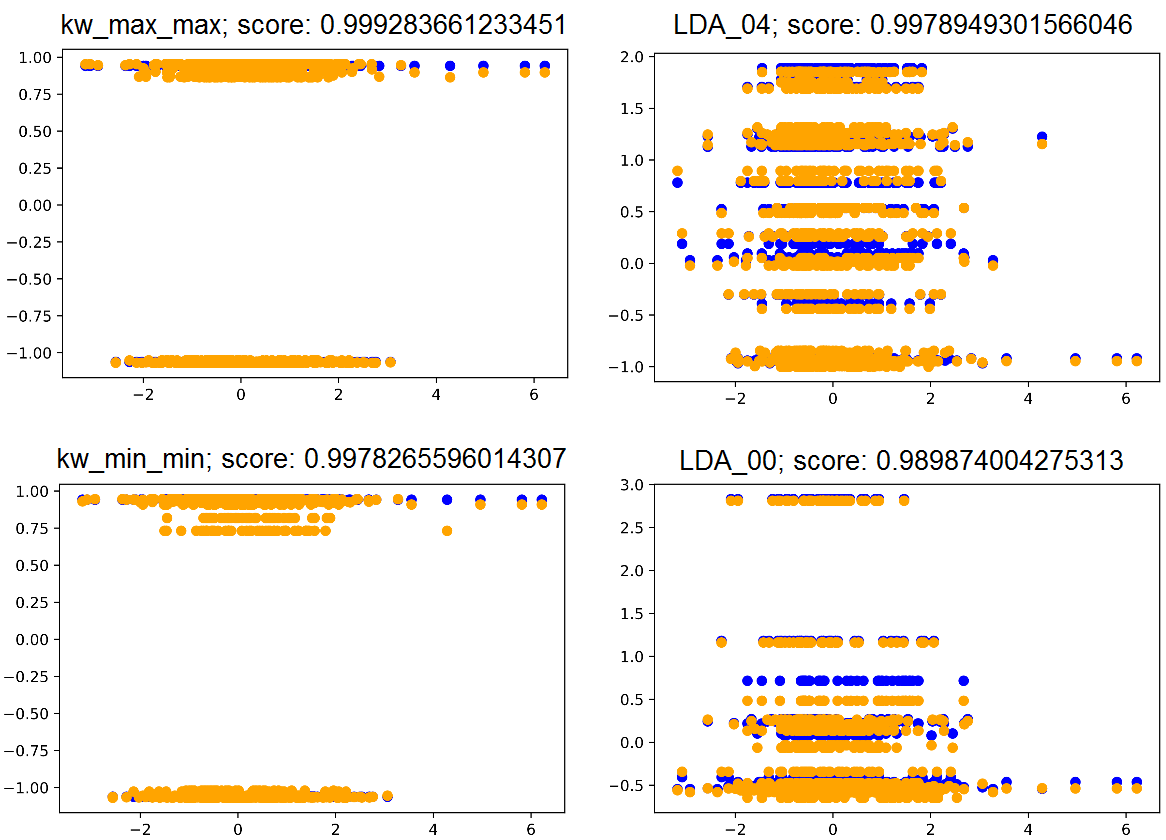
\includegraphics[height=0.7\linewidth]{./figures/best_inversion}
	\caption{The best results of the inversion}
	\label{fig:best_inversion}
\end{figure}
At the representation of the resulted values of inversion, the original ones are colored blue and the inverted values have a color orange.\bigskip

As a summarization it is exciting to see that the best result all came from the combination of almost the same parameters. They are the \textbf{hyperbolic tangent} as activation function, \textbf{L-BFGS} as optimization method, \textbf{0.01} as alpha value and \textbf{0.001} or \textbf{0.0001} as learning rate.\smallskip

It is also an interesting result, that this combination is not equal with the best parameters of the training.